\documentclass{article}

\usepackage{geometry}
\usepackage{amsmath}
\usepackage{graphicx}
\usepackage{listings}
\usepackage{xcolor}
\usepackage{chngcntr}


\geometry{letterpaper, margin=1.5in, bottom=1in}

\counterwithin*{equation}{subsection}

\title{Problem Set Four}
\date{04/03/2018}
\author{Zhixian(Jason) Yu}

\definecolor{mygreen}{rgb}{0,0.6,0}
\definecolor{mygray}{rgb}{0.9,0.9,0.9}
\definecolor{mymauve}{rgb}{0.58,0,0.82}

\lstset{ %
  backgroundcolor=\color{mygray},   % choose the background color
  basicstyle=\footnotesize,        % size of fonts used for the code
  breaklines=true,                 % automatic line breaking only at whitespace
  captionpos=b,                    % sets the caption-position to bottom
  commentstyle=\color{mygreen},    % comment style
  escapeinside={\%*}{*)},          % if you want to add LaTeX within your code
  keywordstyle=\color{blue},       % keyword style
  stringstyle=\color{mymauve},     % string literal style
  keepspaces=true,
  tabsize=2,
  language=Python,
  numbersep=3pt, 
  numbers=left
  %frame=single
}

\begin{document}
\maketitle
\pagenumbering{gobble}
\newpage

\section{Theory}
\subsection*{Problem 1}
After update, the center $C^{(k-1)}$ becomes $C^{(k)}$, and:
\begin{equation*}
C^{(k)} = C^{(k-1)} + \epsilon(x^{(\mu)} - C^{(k-1)})
\end{equation*}
The squared distance between $C^{(k)}$ and $x^{(\mu)}$ is:
\begin{align*}
\| C^{(k)} - x^{(\mu)} \|^2 &= \|C^{(k-1)} + \epsilon(x^{(\mu)} - C^{(k-1)}) - x^{(\mu)} \|^2 \\
&= \|(1-\epsilon)(C^{(k-1)} -  x^{(\mu)}) \|^2 \\
&= (1- \epsilon)^2 \|C^{(k-1)} - x^{(\mu)} \|^2
\end{align*}
Because $\epsilon$ is the learning rate and $0 < \epsilon < 1$, therefore $(1- \epsilon)^2 < 1$ and:
\begin{equation*}
\| C^{(k)} - x^{(\mu)} \|^2 < \|C^{(k-1)} - - x^{(\mu)} \|^2
\end{equation*}
So the update rule moves the winning center closer to the data point.

\subsection*{Problem 2}
Let $C^{(k)}$ be the center after the kth update, and $C^0$ is the random initial value. Let $x^{(\mu_k)}$ be the data value used at the kth update. So we have:
\begin{align*}
C^{(k)} &= C^{(k-1)} + \epsilon_0(x^{(\mu_k)} - C^{(k-1)}) \\
&= (1-\epsilon_0)C^{(k-1)} + \epsilon_0 x^{(\mu_k)} \\
&= (1-\epsilon_0)[(1-\epsilon_0)C^{(k-2)} + \epsilon_0 x^{(\mu_{k-1})}]+ \epsilon_0 x^{(\mu_k)} \\
&= (1-\epsilon_0)^2C^{(k-2)} + \epsilon_0 (1-\epsilon_0) x^{(\mu_{k-1})} + \epsilon_0 x^{(\mu_k)} \\
&= (1-\epsilon_0)^2[(1-\epsilon_0)C^{(k-3)} + \epsilon_0 x^{(\mu_{k-2})}] + \epsilon_0 (1-\epsilon_0) x^{(\mu_{k-1})}+ \epsilon_0 x^{(\mu_k)} \\
&= (1-\epsilon_0)^3C^{(k-3)} + \epsilon_0 (1-\epsilon_0)^2 x^{(\mu_{k-2})} + \epsilon_0 (1-\epsilon_0) x^{(\mu_{k-1})}+ \epsilon_0 x^{(\mu_k)} \\
\vdots \\
&= (1-\epsilon_0)^k C^{(0)} + \sum^{k}_{i=1}\epsilon_0 (1-\epsilon_0)^{i-1} x^{(\mu_{k-i+1})}
\end{align*}
Similarly with previous problem, $0 < \epsilon_0 < 1$, so $(1- \epsilon_0) > (1- \epsilon_0)^2 > (1- \epsilon_0)^3 > \hdots > (1- \epsilon_0)^{k-1}$. Thus the contribution of $x^{\mu_1}$ to $C^{(k)}$ is smaller than $x^{\mu_2}$, that of $x^{\mu_2}$ is smaller than $x^{\mu_3}$, etc. The algorithm gradually forgets previously seen data points. 

\subsection*{Problem 3}
In the base case, learning rate is 1. The equation is obviously true in the following sense:
\begin{equation*}
c^1 = c^0 + 1*(x^{\mu_1} - c^0) = x^{\mu_1}
\end{equation*}
Assume the equation holds for $k-1$:
\begin{equation*}
c^{k-1} = \frac{1}{k-1} \sum^{k-1}_{i=1} x^{(\mu_{k-1})} 
\end{equation*}
The learning rate at the kth step is $\frac{1}{k}$, so:
\begin{align*}
c^{k} &= c^{k-1} + \frac{1}{k}(x^{(\mu_{k})} - c^{k-1}) \\
&= (1- \frac{1}{k}) c^{k-1} + \frac{1}{k}x^{(\mu_{k})} \\
&= \frac{k-1}{k}\frac{1}{k-1} \sum^{k-1}_{i=1} x^{(\mu_{k-1})}  + \frac{1}{k}x^{(\mu_{k})} \\
&= \frac{1}{k}(\sum^{k-1}_{i=1} x^{(\mu_{k-1})} + x^{(\mu_{k})}) \\
&= \frac{1}{k}\sum^{k}_{i=1} x^{(\mu_{k})}
\end{align*}
Therefore the equation holds for any $k$. 

\subsection*{Problem 4}
\paragraph{a)}
If we expand $(B-C)^2$, we get:
\begin{equation*}
(B-C)^2_{ii} = \sum^{n}_{k=1}(B-C)_{ik}(B-C)_{ki}
\end{equation*}
Because both $B$ and $C$ are symmetric matrices, $(B-C)_{ik} = (B-C)_{ki}$. So:
\begin{equation*}
(B-C)^2_{ii} = \sum^{n}_{k=1}(B-C)^2_{ik} = \sum^{n}_{k=1}(B_{ik}-C_{ik})^2
\end{equation*}
Therefore the trace of $(B-C)^2$ is:
\begin{align*}
trace((B-C)^2) &= \sum^{n}_{i=1}(B-C)^2_{ii} \\
&= \sum^{n}_{i=1}\sum^{n}_{k=1}(B_{ik}-C_{ik})^2 \\
&= \sum_{ij}(B_{ij}-C_{ij})^2
\end{align*}

\paragraph{b)} Because both $B$ and $C$ are symmetric matrices, $\Lambda$ and $\hat{\Lambda}$ are real. In addition, $R$ and $S$ are orthonormal basis, satisfying the following conditions:
\begin{equation*}
R^T R = R R^T = I, S^T S =S S^T = I
\end{equation*}
Because $B$ has non-zero eigenvalues, thus diagonal of $\Lambda$ has some positive and negative entries as well as a 0. Because $C$ is positive semi-definite, the diagonal entries of $\Lambda$ are either positive or 0.

\paragraph{c)} From $R^T C R = \hat{\Lambda}$, we get $C=R\hat{\Lambda}R^T$. So:
\begin{align*}
S^TCS &= S^T R\hat{\Lambda}R^T S \\
&= (S^T R) \hat{\Lambda} (S^T R)^T
\end{align*}
Let $G=S^T R$. We have:
\begin{equation*}
G^T G = R^T S S^T R = I
\end{equation*}
Therefore $S^TCS = G \hat{\Lambda} G^T$, and $G$ is a orthogonal matrix. 

\paragraph{d)} From the spectral theorem, we know that $B = S \Lambda S^T$. From question c), we know that $C = S(G \hat{\Lambda} G^T)S^T$. Therefore:
\begin{align*}
trace(B-C)^2 &= trace[S \Lambda S^T - S(G \hat{\Lambda} G^T)S^T]^2 \\
&= trace[S (\Lambda- G \hat{\Lambda} G^T)S^T]^2 \\
&= trace[S (\Lambda- G \hat{\Lambda} G^T)S^T S (\Lambda- G \hat{\Lambda} G^T)S^T] \\
&= trace[S (\Lambda- G \hat{\Lambda} G^T)^2 S^T] \\
&= trace[(\Lambda- G \hat{\Lambda} G^T)^2 S^T S]\\
&= trace(\Lambda- G \hat{\Lambda} G^T)^2
\end{align*}

\paragraph{e)} We can expand $trace((\Lambda - G \hat{\Lambda} G^T)^2)$ as following:
\begin{align*}
trace((\Lambda - G \hat{\Lambda} G^T)^2) &= trace(\Lambda^2 - \Lambda G \hat{\Lambda} G^T - G \hat{\Lambda} G^T \Lambda + (G \hat{\Lambda} G^T)^2) \\
&= trace(\Lambda^2 - \Lambda G \hat{\Lambda} G^T - G \hat{\Lambda} G^T \Lambda + (G \hat{\Lambda} G^T)(G \hat{\Lambda} G^T))\\
&= trace(\Lambda^2 - \Lambda G \hat{\Lambda} G^T - G \hat{\Lambda} G^T \Lambda + G \hat{\Lambda} \hat{\Lambda} G^T) \\
&= trace(\Lambda^2) - 2trace(\Lambda G \hat{\Lambda} G^T) + trace(G \hat{\Lambda}^2 G^T) \\
&= trace(\Lambda^2) - 2trace(\Lambda G \hat{\Lambda} G^T) + trace(\hat{\Lambda}^2)
\end{align*}
To minimize $trace((\Lambda - G \hat{\Lambda} G^T)^2)$, we need to maximize $trace(\Lambda G \hat{\Lambda} G^T)$. Let $\lambda_i, i \in [1, n]$ be the diagonal elements of $\Lambda$, and $\hat{\lambda}_i, i \in [1, n]$ be the diagonal elements of $\hat{\Lambda}$. \newline Because $\Lambda$ is a diagonal matrix, $(\Lambda G \hat{\Lambda} G^T)_{ii} = \Lambda_{ii} (G \hat{\Lambda} G^T)_{ii} = \lambda_i (G \hat{\Lambda} G^T)_{ii}$, so:
\begin{align*}
trace(\Lambda G \hat{\Lambda} G^T) &= \sum^{n}_{i=1}\lambda_i(G \hat{\Lambda} G^T)_{ii}
\end{align*}
We can further expand $(G \hat{\Lambda} G^T)_{ii}$, and the previous equation becomes:
\begin{align*}
trace(\Lambda G \hat{\Lambda} G^T) &= \sum^{n}_{i=1}\lambda_i(\sum^{n}_{j=1} G^2_{ij} \hat{\lambda}_j) \\
&= \sum^{n}_{i=1}\lambda_i(\sum^{n}_{j \ne i} G^2_{ij} \hat{\lambda}_j + G^2_{ii}\hat{\lambda}_i) \\
&= \sum^{n}_{i=1}\lambda_i[\sum^{n}_{j \ne i} G^2_{ij} \hat{\lambda}_j + (1 - \sum^{n}_{j \ne i} G^2_{ij})\hat{\lambda}_i] \\
&= \sum^{n}_{i=1}\lambda_i(\hat{\lambda}_i + \sum^{n}_{j \ne i} G^2_{ij} \hat{\lambda}_j - \hat{\lambda}_i)
\end{align*}


\subsection*{Problem 5}
The goal is to solve $Ly=\lambda D y$. In addition, $L = D-W$ and $D_{ii} = \sum_{j} W_{ij}$. Suppose $L$ is a $n*n$ matrix. We can show that zero is always an eigenvalue and the associated eigenvector is $e$ which has the length of $n$ and $e_i = 1, i \in [1, n]$. For any $i \in [1,n]$, we have:
\begin{align*}
(Le)_i &= \sum^{n}_{j=1} L_{ij} \\
&= \sum^{n}_{j=1} (D_{ij} - W_{ij}) \\ 
&= \sum^{n}_{j=1} D_{ij} - \sum^{n}_{j=1}W_{ij} \\
&= D_{ii} - \sum^{n}_{j=1}W_{ij} \\
&= \sum_{j} W_{ij} - \sum^{n}_{j=1}W_{ij} \\
&= 0
\end{align*}
Therefore $Le =0 = 0De$. Zero is always an eigenvalue and the associated eigenvector is a vector of ones. 


\newpage
\section{Programming}
The following code sets up the environment and import packages.
\begin{lstlisting}
	import numpy as np
	import matplotlib.pyplot as plt
	import matplotlib.image as mpimg
	import cv2
	import random
\end{lstlisting}

\subsection*{Problem 1}
The following code reads image from file, and makes the color ranging from 0 to 1 instead of 0 to 255.  
\begin{lstlisting}
	img = mpimg.imread('./data/Penguins.jpg')
	img = img/255
\end{lstlisting}
First thing is to randomly initialize 10 centers. The colors of the 10 random centers are shown in figure~\ref{fig:1_random_center}.
\begin{lstlisting}
	centers = [np.random.rand(3) for i in range(10)]  # randomly intialize 10 centers
	for i in range(10):
		plt.subplot(3,4,i+1)
		plt.imshow(np.tile(centers[i], (10, 10, 1)))
	plt.plot()
\end{lstlisting}

\begin{figure}[h!]
\centering
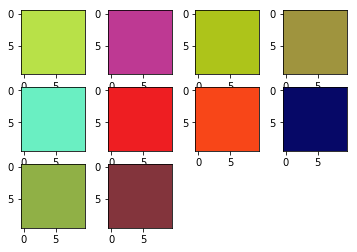
\includegraphics[width=0.6\linewidth]{../images/1_random_center.png}
\caption{10 random colors that were initially picked.}
\label{fig:1_random_center}
\end{figure}

The following code executes the LBG clustering algorithm. It was iterated 100 times. 
\begin{lstlisting}
	pixel_center_mapping = np.zeros((img.shape[0], img.shape[1])).astype(np.int8)
	for i in range(100):
		voronoi_set_sum = np.zeros((10,3))
		voronoi_set_cnt = np.array([0 for i in range(10)])
		for i in range(img.shape[0]):
			for j in range(img.shape[1]):
				distances = [np.linalg.norm(centers[k] - img[i][j]) for k in range(10)]
				closest_ind = np.argmin(distances)
				pixel_center_mapping[i][j] = closest_ind
				voronoi_set_sum[closest_ind] += img[i][j]
				voronoi_set_cnt[closest_ind] += 1
		for i in range(10):
			if voronoi_set_cnt[i] != 0:
				centers[i] = voronoi_set_sum[i]/voronoi_set_cnt[i]
\end{lstlisting}
After clustering, the center colors are shown in figure~\ref{fig:1_trained_center}.
\begin{lstlisting}
	for i in range(10):
		plt.subplot(3,4,i+1)
		plt.imshow(np.tile(centers[i], (10, 10, 1)))
	plt.plot()
\end{lstlisting}

\begin{figure}[h!]
\centering
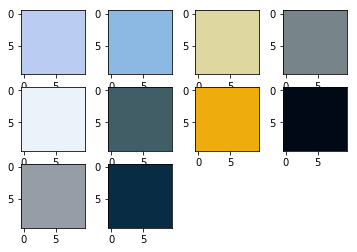
\includegraphics[width=0.6\linewidth]{../images/1_trained_center.png}
\caption{10 center colors after LBG clustering.}
\label{fig:1_trained_center}
\end{figure}

The following code is used to produce the color-quantized new picture, which is shown in figure~\ref{fig:1_new_penguin}. As is shown, the sky was approximately quantized to 3 regions, and the penguins are quantized to about 4-5 colors. 
\begin{lstlisting}
	new_img = np.copy(img)
	for i in range(img.shape[0]):
		for j in range(img.shape[1]):
			new_img[i][j] = centers[pixel_center_mapping[i][j]]
	plt.imshow(new_img)
	plt.show()
\end{lstlisting}

\begin{figure}[h!]
\centering
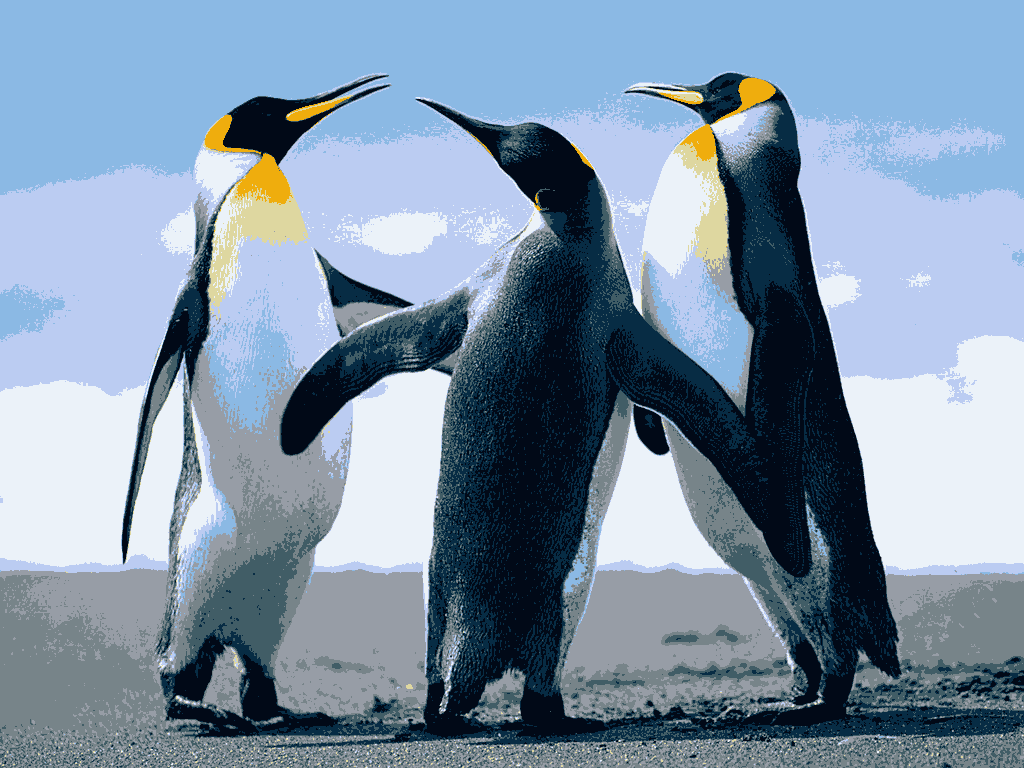
\includegraphics[width=0.6\linewidth]{../images/1_new_penguin.png}
\caption{Color quantized image.}
\label{fig:1_new_penguin}
\end{figure}

\subsection*{Problem 2}
The following code defines the SOM function to execute SOM algorithm.
\begin{lstlisting}
	def r(n, T):
		return 0.9*(1-n/T)
		
	def epsi(n, T):
		return 0.9*(1-n/T)

	def h(x, n, T):
		return np.exp(-x**2/r(n, T)**2)

	def find_winning_c(x, E):
		min_dist= np.linalg.norm(x-E[0])
		min_ind = 0
		for i in range(1, E.shape[0]):
			if np.linalg.norm(x-E[i]) < min_dist:
				min_ind = i
				min_dist = np.linalg.norm(x-E[i])
		return min_ind

	def SOM(X, n_iterations=10000, dim=1):
		X = np.array(X)
		N = X.shape[0] # shape 0 is the number of elements
		E = np.random.rand(N, dim) # pick random centers
		for i in range(n_iterations):
			x = X[random.randrange(N)]
	#         print(x)
			c = find_winning_c(x, E)
			# update E
			for j in range(N):
				E[j] = E[j] + epsi(i, n_iterations)*h((c-j), i, n_iterations)*(x-E[j])
	#         print(E)
		return E
\end{lstlisting}
Using the data provided, it is able to perfectly reconstructs the original data. Here are the parameter settings: $\epsilon(n) = r(n) = 0.9(1-\frac{n}{T})$ where $T=10000$ which is the total number of iterations. The result is plotted in figure~\ref{fig:2}. The blue dots represent original data while the red dots represent reconstructed data points. They match perfectly. According to the discussion in class, it seems important to choose a higher number of iterations. Here $10000$ is enough. 
\begin{lstlisting}
	X = [0.34, 0.12, 0.73, 0.97, 0.07, 0.56]
	SOM(X)
	plt.plot(SOM(X), np.zeros(6), 'r.', label='SOM')
	plt.plot(X, np.ones(6), 'b.', label='Original')
	plt.legend()
	plt.show()
\end{lstlisting}

\begin{figure}[h!]
\centering
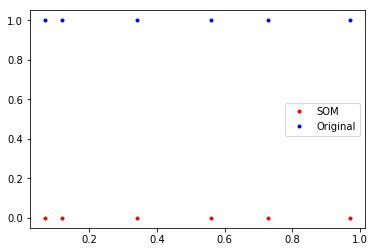
\includegraphics[width=0.6\linewidth]{../images/2.png}
\caption{Original and SOM-reconstructed data.}
\label{fig:2}
\end{figure}

\subsection*{Problem 3}
The following code reads the animal data. 
\begin{lstlisting}
	animals = ['Dove','Hen','Duck','Goose','Owl','Hawk','Eagle','Fox','Dog','Wolf','Cat','Tiger','Lion','Horse','Zebra','Cow']
	features = ['small size','medium size','large size','2 legs','4 legs','hair','hooves','mane','feathers','hunts','runs','flys','swims']

	M = [[1 ,1 ,1 ,1 ,1 ,1 ,0 ,0 ,0 ,0 ,1 ,0 ,0 ,0 ,0 ,0],[
	0 ,0 ,0 ,0 ,0 ,0 ,1 ,1 ,1 ,1 ,0 ,0 ,0 ,0 ,0 ,0],[
	0 ,0 ,0 ,0 ,0 ,0 ,0 ,0 ,0 ,0 ,0 ,1 ,1 ,1 ,1 ,1],[
	1 ,1 ,1 ,1 ,1 ,1 ,1 ,0 ,0 ,0 ,0 ,0 ,0 ,0 ,0 ,0],[
	0 ,0 ,0 ,0 ,0 ,0 ,0 ,1 ,1 ,1 ,1 ,1 ,1 ,1 ,1 ,1],[
	0 ,0 ,0 ,0 ,0 ,0 ,0 ,1 ,1 ,1 ,1 ,1 ,1 ,1 ,1 ,1],[
	0 ,0 ,0 ,0 ,0 ,0 ,0 ,0 ,0 ,0 ,0 ,0 ,0 ,1 ,1 ,1],[
	0 ,0 ,0 ,0 ,0 ,0 ,0 ,0 ,0 ,1 ,0 ,0 ,1 ,1 ,1 ,0],[
	1 ,1 ,1 ,1 ,1 ,1 ,1 ,0 ,0 ,0 ,0 ,0 ,0 ,0 ,0 ,0],[
	0 ,0 ,0 ,0 ,1 ,1 ,1 ,1 ,0 ,1 ,1 ,1 ,1 ,0 ,0 ,0],[
	0 ,0 ,0 ,0 ,0 ,0 ,0 ,0 ,1 ,1 ,0 ,1 ,1 ,1 ,1 ,0],[
	1 ,0 ,0 ,1 ,1 ,1 ,1 ,0 ,0 ,0 ,0 ,0 ,0 ,0 ,0 ,0],[
	0 ,0 ,1 ,1 ,0 ,0 ,0 ,0 ,0 ,0 ,0 ,0 ,0 ,0 ,0 ,0]]
\end{lstlisting}
Another SOM() function is defined to produce data points in two dimensions. 
\begin{lstlisting}
	def r(n, T):
		return 0.9*(1-n/T)
		
	def epsi(n, T):
		return 0.9*(1-n/T)

	def h(x, n, T):
		return np.exp(-x**2/r(n, T)**2)

	def find_winning_c(x, E):
		min_dist= np.linalg.norm(x-E[0][0])
		min_ind_i = 0
		min_ind_j = 0
		for i in range(E.shape[0]):
			for j in range(E.shape[1]):
				if np.linalg.norm(x-E[i][j]) < min_dist:
					min_ind_i = i
					min_ind_j = j
					min_dist = np.linalg.norm(x-E[i][j])
		return min_ind_i, min_ind_j

	def SOM(X, labels, n_iterations=10000):
		X = np.array(X)
		N = X.shape[0] # shape 0 is the number of elements
		n_features = X.shape[1]
		E = np.random.rand(4, 4, n_features)
		classes = [[0 for i in range(4)] for j in range(4)]
		for i in range(n_iterations):
			presenting_ind = random.randrange(N)
			x = X[presenting_ind]
	#         print(x)
			c = find_winning_c(x, E)
			classes[c[0]][c[1]] = labels[presenting_ind]
			# update E
			for j in range(4):
				for k in range(4):
					dist_index = np.linalg.norm(np.array((j, k)) - np.array(c))
					E[j][k] = E[j][k] + epsi(i, n_iterations)*h(dist_index, i, n_iterations)*(x-E[j][k])
	#         print(E)
		return E, classes
\end{lstlisting}
We can use the defined SOM() function to view the animal data in two dimensions. 
\begin{lstlisting}
	_, som_animal = SOM(np.array(M).T, animals)


	for i in som_animal:
		for j in i:
			print(j, end='\t')
		print('\n')
\end{lstlisting}
The result is shown below. As we can see, it classifies the animals reasonably well. The right side of the table is full of birds-like animals, and the left side is mammals. The lower left part of the table is large animals, and the lower right part of the table is birds that cannot fly. 
\begin{center}
\begin{tabular}{c c c c}
Cat & Fox & Eagle & Hawk \\
Wolf & Dog & Eagle & Dove \\
Lion & Tiger & Hen & Duck \\
Horse & Cow & Hen & Goose 
\end{tabular}
\end{center}

\subsection*{Problem 4}
The following code is used to compute a weight matrix $W$. Nearest neighbor is used and connected neighbors have distance of 1. 
\begin{lstlisting}
	from scipy.spatial import distance_matrix

	def is_nn(i, j, dist_m, n):
		if i == j:
			return 0
		res = 0
		dist_tmp = np.sort(dist_m[i])
		if dist_m[i][j] <= dist_tmp[n]:
			res = 1
			return res
		dist_tmp = np.sort(dist_m[j])
		if dist_m[i][j] <= dist_tmp[n]:
			res = 1
		return res

	def w_construction(X, n):
		X = np.array(X) # samples x features
		N = X.shape[0]
		W = np.zeros((N, N)) - 1
		dist_m = distance_matrix(X, X)
	#     print(dist_m)
		
		for i in range(N):
			for j in range(N):
				if W[j][i] != -1:
					W[i][j] = W[j][i]
				else:
					W[i][j] = is_nn(i, j, dist_m, n)
		
		return W
\end{lstlisting}
The animal data from last question is used. The number of nearest neighbors is chosen as 3 here. We can also view the result in 2 dimensions. 
\begin{lstlisting}
	W = w_construction(np.array(M).T, 3)
	D = np.diag(np.sum(W, axis=0))
	L = D -W
	w, v = np.linalg.eig(np.linalg.inv(D)@L)
	
	# view result	
	plt.figure(figsize=(16,8))
	plt.plot(v[8], v[3], '.')
	for i in range(16):
		plt.text(v[8][i], v[3][i], animals[i])
	plt.show()
\end{lstlisting}
The result is shown in figure~\ref{fig:4_n=3}. As we can see, there are mainly two groups: a horizontal line and a vertical line. The horizontal line represents mammals while the vertical line represents birds. However, some of the mapping is not very accurate. For example, lion and tiger are very far away, although intuitively they should be close. 

\begin{figure}[h!]
\centering
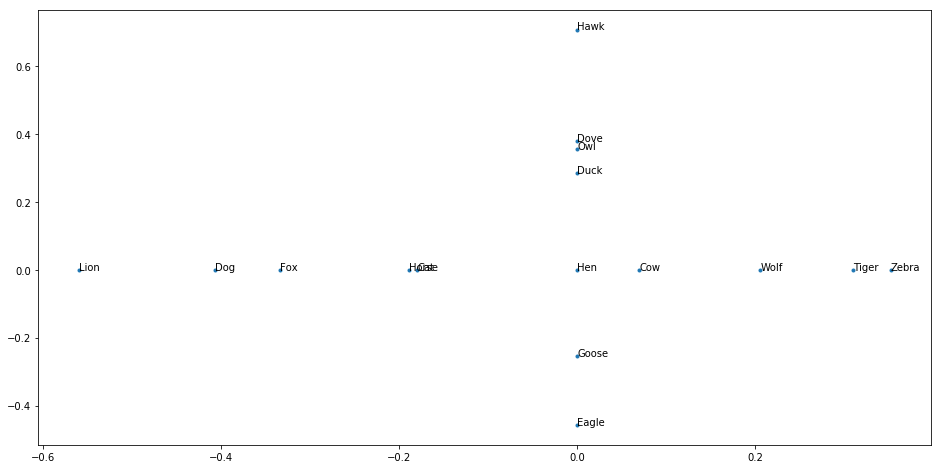
\includegraphics[width=0.6\linewidth]{../images/4_n=3.png}
\caption{Represented 2-D animal data from Laplacian eigenmap dimension reduction method ($n=3$).}
\label{fig:4_n=3}
\end{figure}

If we increase the threshold for choosing nearest neighbors to 7, we get the following figure~\ref{fig:4_n=7}. In this case, some mappings make sense, such as lion and tiger. However, the separation between mammals and birds are not so obvious. In addition, some different animals are mapped together to the same point. This is probably because increasing the threshold produces more connections between different data, therefore some of them lack sufficient neighborhood information to distinguish them apart.

\begin{figure}[h!]
\centering
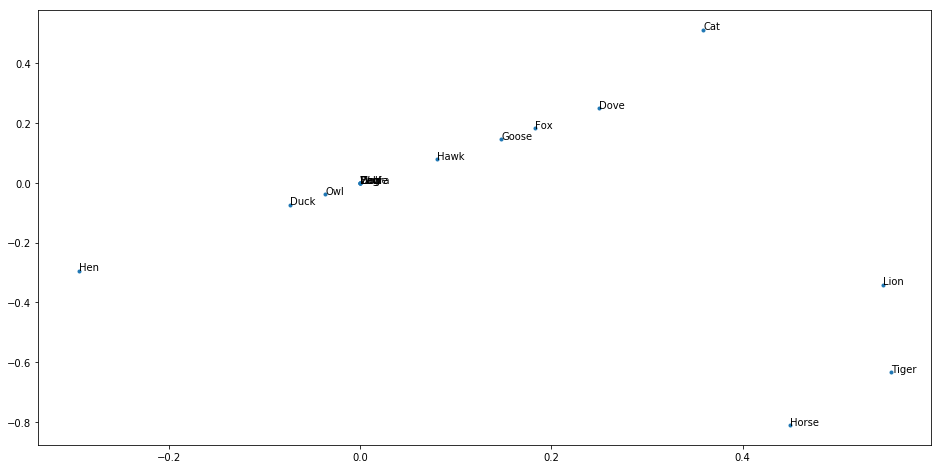
\includegraphics[width=0.6\linewidth]{../images/4_n=7.png}
\caption{Represented 2-D animal data from Laplacian eigenmap dimension reduction method ($n=7$).}
\label{fig:4_n=7}
\end{figure}

\end{document}
